\label{sec:4.4}
%%%%%%%%%%%%%%%%%%%%%%%%%%%%%%%%%%%%%%%%%%%%%%%%%%%%%%%
%(GAO) Calibration pulser
%%%%%%%%%%%%%%%%%%%%%%%%%%%%%%%%%%%%%%%%%%%%%%%%%%%%%%%
The LArASIC has an internal 6-bit DAC to generate a voltage step through a charge injection 
capacitor for calibration. Figure~\ref{fig:calibpulse} shows the pulse response of channel 0 at 
room temperature.  LArASIC is configured with 14 mV/fC gain, 2.0 $\mu$s shaping time, 
900mV baseline, output buffer off, DC coupling and 500pA leakage current. ColdADC is configured 
with single-ended input, BGR reference and 16-bit calibrated data. The observed non-linearity of 
0.19% is dominated by the non-linearity of the 6-bit DAC. The non-linearity of LArASIC and 
ColdADC is expected to be less than 0.1\%.   
\begin{figure}[h!]
\centering
  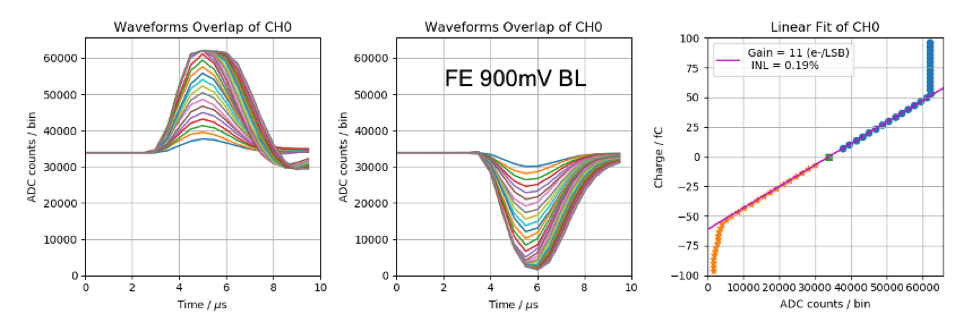
\includegraphics[width=1.0\linewidth]{figures/calibpulse.png}
  \caption{Response of LArASIC + ColdADC to the calibration pulse.}
  \label{fig:calibpulse}
\end{figure}

